% ***************************************** SYMBOLS
\def\abs#1{\lvert#1\rvert}
\def\argdot{{\hspace{0.18em}\cdot\hspace{0.18em}}}
\def\avg#1{\left\{#1\right\}_\omega}
\def\D{{\tn D}}
\def\div{\operatorname{div}}
\def\Eh{\mathcal E_h}       % edges of \Th
\def\Ehcom{\mathcal E_{h,C}}         % edges of \Th on interface with lower dimension
\def\Ehdir{\mathcal E_{h,D}}         % Dirichlet edges of \Th
\def\Ehint{\mathcal E_{h,I}}       % interior edges of \Th
\def\grad{\nabla}
\def\jmp#1{[#1]}
\def\n{\vc n}
\def\vc#1{\mathbf{\boldsymbol{#1}}}     % vector
\def\R{\mathbb R}
\def\sc#1#2{\left(#1,#2\right)}
\def\Th{\mathcal T_h}       % triangulation
\def\th{\vartheta}
\def\tn#1{{\mathbb{#1}}}    % tensor
\def\Tr{\operatorname{Tr}}
\def\where{\,|\,}
%***************************************************************************

\section{Reaction Term in Transport}
\label{sec:reaction_term}

The {\tt TransportOperatorSplitting} method supports the reaction term $F_R(c^1,\ldots,c^s)$ on the right hand side of the equation (\ref{e:ADE}).
It can represent several models of chemical or physical nature. 
Figure \ref{fig:reaction_term} shows all possible reactional models that we support in combination with the transport process. The Operator Splitting method enables 
us to deal with the convection part and reaction term side by side. The convected quantities do not influence each other in the convectional
process and are balanced over the elements. On the other hand the reaction term relates the convected quantities and can be computed 
separately on each element.

We move now to the description of the reaction models which can be seen again in Figure \ref{fig:reaction_term}. 
The convected quantity is considered to be the concentration of substances. 
Up to now we can have \emph{dual porosity}, \emph{sorption} (these two are more of a physical nature) and (chemical) \emph{reaction} models in the reaction term. 

\begin{figure}
  \centering
  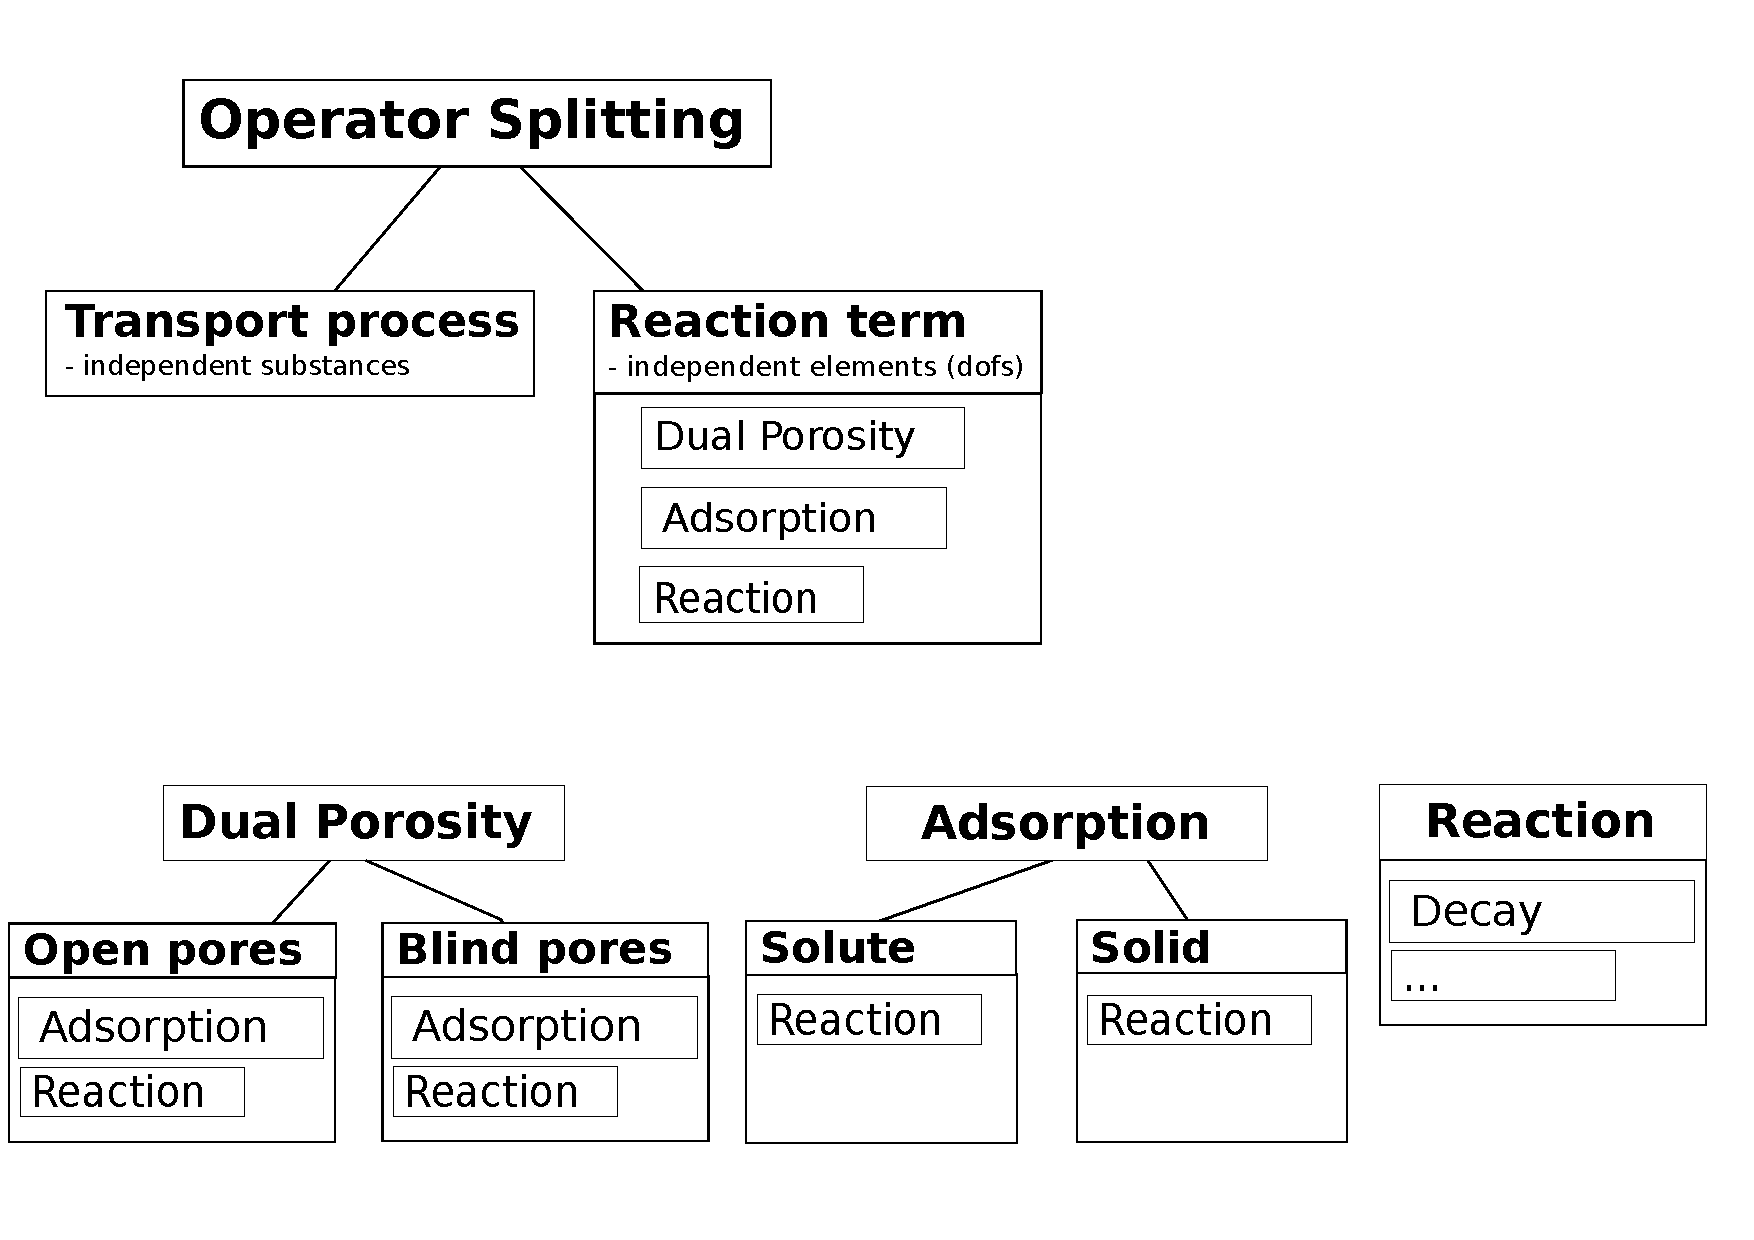
\includegraphics[width=\textwidth]{\fig/reaction_term.pdf}
  \caption{The scheme of the reaction term objects. The lines represents connections between different models. 
  The tables under model name include the possible models which can be connected to the model above.}
  \label{fig:reaction_term}
\end{figure}

The \emph{reaction} model acts only on the specified substances and computes exchange of concentration 
among them. It does not have its own output because it only changes the concentration of substances 
in the specified zone where the reaction takes place. See \ref{sec:linear_reactions} for thorough description.

The \emph{sorption} model describes the exchange of concentration of the substances between liquid and solid. It can be
followed by another \emph{reaction} that can run in both phases. The concentration in solid is an additional output 
of this model. See Subsection \ref{sec:sorp_math}.


The \emph{dual porosity} model, described in Subsection \ref{sec:dual_porosity}, introduces the so called immobile (or dead-end) pores in the matrix. The convection process operates only on the concentration of the substances in the mobile zone (open pores) 
and the exchange of concentrations from/to immobile zone is governed by molecular diffusion. This process can be followed by 
\emph{sorption} model and/or chemical \emph{reaction}, both in mobile and immobile zone. The immobile concentration is an
additional output.


\subsection{Dual Porosity}
\label{sec:dual_porosity}

Up to now we have described the transport equation for the single porosity model. The dual porosity model splits the mass into 
two zones -- the mobile zone and the immobile zone. Both occupy the same macroscopic volume, however on the microscopic scale, 
the immobile zone is formed by the dead-end pores, where the liquid is trapped and cannot pass through. The rest of the pore volume 
is occupied by the mobile zone. Since the liquid in the immobile pores is immobile, the exchange of the substance is only due 
to molecular diffusion. We consider simple nonequilibrium linear model:
\begin{align}
    \vartheta_m \partial_t c_m &= D_{dp} ( c_i - c_m), \label{eqn:dual_porosity_ode1}\\
    \vartheta_i \partial_t c_i &= D_{dp} ( c_m - c_i), \label{eqn:dual_porosity_ode2}
\end{align}
where $c_m$ is the concentration in the mobile zone, $c_i$ is the concentration in the immobile zone and
\hyperA{DualPorosity-Data::diffusion-rate-immobile}{$D_{dp}$} is a diffusion rate between the zones.
\hyperA{DualPorosity-Data::porosity-immobile}{$\vartheta_i$}~denotes porosity of the immobile zone  and 
$\hyperlink{TransportOperatorSplitting-Data::porosity::B}{\vartheta_m} = \vartheta$ the mobile porosity from transport equation \eqref{e:ADE}.

The analytic solution of the system of differential equations at the time $t$ with initial conditions $c_m(0)$ and $c_i(0)$ is
\begin{align}
     c_m(t) &= (c_m(0) - c_a(0)) \exp\left(- D_{dp}\left(\frac{1}{\vartheta_m} + \frac{1}{\vartheta_i}\right) t \right) + c_a(0), 
     \label{eqn:dual_porosity_anal1}\\
     c_i(t) &= (c_i(0) - c_a(0)) \exp\left(- D_{dp}\left(\frac{1}{\vartheta_m} + \frac{1}{\vartheta_i}\right) t \right) + c_a(0),
     \label{eqn:dual_porosity_anal2}
\end{align}
where $c_a$ is the weighted average
\[
  c_a = \frac{\vartheta_m c_m + \vartheta_i c_i}{\vartheta_m + \vartheta_i}.
\]

If the time step is large, we use the analytic solution to compute new values of concentrations. 
Otherwise, we replace the time derivatives in \eqref{eqn:dual_porosity_ode1} and \eqref{eqn:dual_porosity_ode2} 
by first order forward differences and we get the classical Euler scheme
\begin{align}
  c_m(t^+) = \frac{D_{dp} \Delta t}{\vartheta_m}(c_i(t) - c_m(t)) + c_m(t), \\
  c_i(t^+) = \frac{D_{dp} \Delta t}{\vartheta_i}(c_m(t) - c_i(t)) + c_i(t), \\
\end{align}
where $\Delta t = t^+ - t$ is the time step. 

The condition on the size of the time step is derived from the Taylor expansion of 
\eqref{eqn:dual_porosity_anal1} or \eqref{eqn:dual_porosity_anal2}, respectively. We neglect the higher order 
terms and we want the second order term to be smaller than the given scheme tolerance 
\hyperA{DualPorosity::scheme-tolerance}{$tol$}, relatively to $c_a$,
\begin{equation}
  (c_m(0) - c_a(0))
  \frac{ D_{dp}^2 (\Delta t)^2 \left(\frac{\vartheta_m + \vartheta_i}{\vartheta_m \vartheta_i}\right)^2}{2}
  \frac{1}{c_a} \leq tol. \\
\end{equation}
We then transform the above inequation into the following condition which is tested in the program
\begin{equation} \label{eqn:euler_scheme_condition}
  \max(|c_m(0) - c_a(0)|, |c_i(0) - c_a(0)|) \leq 
  2 c_a \left(\frac{\vartheta_m \vartheta_i}{D_{dp} \Delta t (\vartheta_m + \vartheta_i)}\right)^2 tol. \\
\end{equation}
If the inequation \eqref{eqn:euler_scheme_condition} is not satisfied, then the analytic 
solution is used.
 

\subsection{Equilibrial Sorption}
\label{sec:sorp_math}

The simulation of monolayer, equilibrial sorption is based on the solution of two algebraic equations, namely the mass balance (in unit volume)
\begin{equation}
\label{eq:mass_balance_sorption}
\th \varrho_l c_l + (1-\th) \varrho_s M_s c_s = c_T = const.
\end{equation}
and an empirical sorption law
\begin{equation}
\label{eq:relation_cs_cl}
c_s = f(c_l),
\end{equation}
given in terms of the so-called isotherm $f$.
Its form is determined by the parameter \hyperA{Sorption-Data::sorption-type}{\tt sorption\_type}:
\begin{itemize}
 \item ``$none$'': $f(c_l)=0$ (the sorption model returns zero concentration in solid);
 \item ``$linear$'': $f(c_l) = k_l c_l$;
 \item ``$freundlich$'': $f(c_l) = k_F c_l^{\alpha}$;
 \item ``$langmuir$'': $f(c_l) = k_L \frac{\alpha c_l}{1 + \alpha c_l}$.
       Langmuir isotherm has been derived from thermodynamic laws. $k_L$ denotes the maximal amount 
       of sorbing specie which can be kept in an unit volume of a bulk matrix. Coefficient $\alpha$ is 
       a fraction of sorption and desorption rate constant $\alpha = \frac{k_a}{k_d}$.
\end{itemize}

Notation:
\begin{itemize}
 \item In solid, $c_s = \frac{n}{m_s}$ [mol\,$\mathrm{kg}^{-1}$] is the fraction of the molar amount of the solute 
       adsorbed $n$ and the amount of the adsorbent $m_s$ (mass of solid), all in unit volume.
 \item In liquid, $c_l = \frac{m}{m_l}$ \units{}{}{} is the fraction of the amount of the solute $m$ and 
       the mass of liquid $m_l$, all in unit volume. The relation between $c_l$ and the concentration $c$ from 
       transport equation \eqref{e:ADE} is $c = c_l \varrho_l$.
 \item \hyperA{Sorption::solvent-density}{$\varrho_l$}, \hyperA{Sorption-Data::rock-density}{$\varrho_s$} is the liquid (solvent) density and the solid (rock) density, respectively.
 \item \hyperA{Sorption::molar-mass}{$M_s$} denotes the molar mass of a substance.
 \item Multiplication parameters $k_i, i\in\{ l,F,L\}$ [mol\,$\mathrm{kg}^{-1}$] are given by 
       \hyperA{Sorption-Data::isotherm-mult}{\tt isotherm\_mult}.
 \item Additional parameter $[\alpha] = 1$ is given by \hyperA{Sorption-Data::isotherm-other}{\tt isotherm\_other}.
\end{itemize}

The units of $c_l$, $c_s$ and $k_i$ can vary in literature. To avoid misinterpretation, we derive (according
to Bowman~\cite{bowman_conversion_1982}) a conversion rule for Freundlich isotherm which will lead the user 
also in other cases, we believe. 

Let us have $c$ \units{1}{-3}{}, the mass concentration in liquid, and $s$ [kg\,$\mathrm{kg}^{-1}$], 
the fraction of the amount of the solute adsorbed and the amount of the adsorbent in solid. 
The unit of $K$ follows from the dimensional analysis of $s=Kc^{\alpha}$:
\[[K] = \frac{\rm{kg}^{1-\alpha}\rm{m}^{3\alpha}}{\rm{kg}},\]
which we want to convert to $k_F$ [mol\,$\mathrm{kg}^{-1}$] in the formula $c_s=k_Fc_l^\alpha$.

The first step is a conversion of the mass of the solute to moles by dividing it by the
molar mass $M_s$. We then have the formula 
\begin{eqnarray}
s&=&Kc^{\alpha} \nonumber \\
\frac{s}{M_s} &=& K'\left(\frac{c}{M_s}\right)^\alpha, \label{eqn:sorp_molar_conc}\\
s &=& K'M_s^{1-\alpha}c^\alpha, \nonumber 
\end{eqnarray}
where $s=c_sM_s$ and $K'=KM_s^{\alpha-1}$ [$\rm{mol}^{1-\alpha}\rm{kg}^{-1}\rm{m}^{3\alpha}$] is a new constant,
distributing the molar concentration in liquid to the ratio of the molar mass and the amount of sorbent in solid.

The second step is introducing $c_l = \frac{c}{\varrho_l}$ into the formula \eqref{eqn:sorp_molar_conc}
\begin{equation}
c_s = K'\left(\frac{c_l \rho_l }{M_s}\right)^\alpha
= K' M_s^{-\alpha}\rho_l^{\alpha}c_l^\alpha 
= \left( K M_s^{-1}\rho_l^{\alpha} \right) c_l^\alpha,
\end{equation}
where we can denote 
\begin{equation}
k_F=K M_s^{-1}\rho_l^{\alpha},
\end{equation} 
which is the constant we are looking for. This can be also translated to the case of the linear isotherm, where
$\alpha=1$ and $[K] = \rm{kg}^{-1}\rm{m}^{3}$, and we get the conversion rule
\begin{equation}
k_l=K M_s^{-1}\rho_l.
\end{equation} 
The conversion of different prefixes of units are left on the user. One should be careful using the 
Freundlich isotherm, though, where the exponent $\alpha$ must not be forgotten.

Let us now describe the actual computation of the sorption model. Denoting
\[ \mu_l = \varrho_l \th, \quad \mu_s = M_s \varrho_s\cdot(1-\th), \]
and using \eqref{eq:relation_cs_cl}, the mass balance \eqref{eq:mass_balance_sorption} reduces to the equation
\begin{equation}
 c_T = \mu_l c_l + \mu_s f(c_l),
 \label{eq:nonlin_sorption}
\end{equation}
which can be either solved iteratively or using interpolation.
To solve \eqref{eq:nonlin_sorption} iteratively, it is very important to define the interval where 
to look for the solution (unknown $c_l$), see Figure \ref{fig:sorpce}. The lower bound is $0$ (concentration can not reach negative values). 
The upper bound is derived using a simple mapping. Let us suppose limmited 
\hyperA{Sorption::solubility}{$solubility$} of the selected transported substance and let us denote the 
limmit $\bar{c}_l$. We keep the maximal "total mass" 
$\bar{c}_T= \mu_l\cdot \bar{c}_l + \mu_s\cdot f(\bar{c}_l)$, but we dissolve all the mass to get 
maximal $c_l^{max} > \bar{c}_l$. That means $c_s = 0$ at this moment. We can slightly enlarge the interval by setting the upper bound equal to 
$c_l^{max} + const_{small}$.

\begin{figure}[ht!]
 \centering
 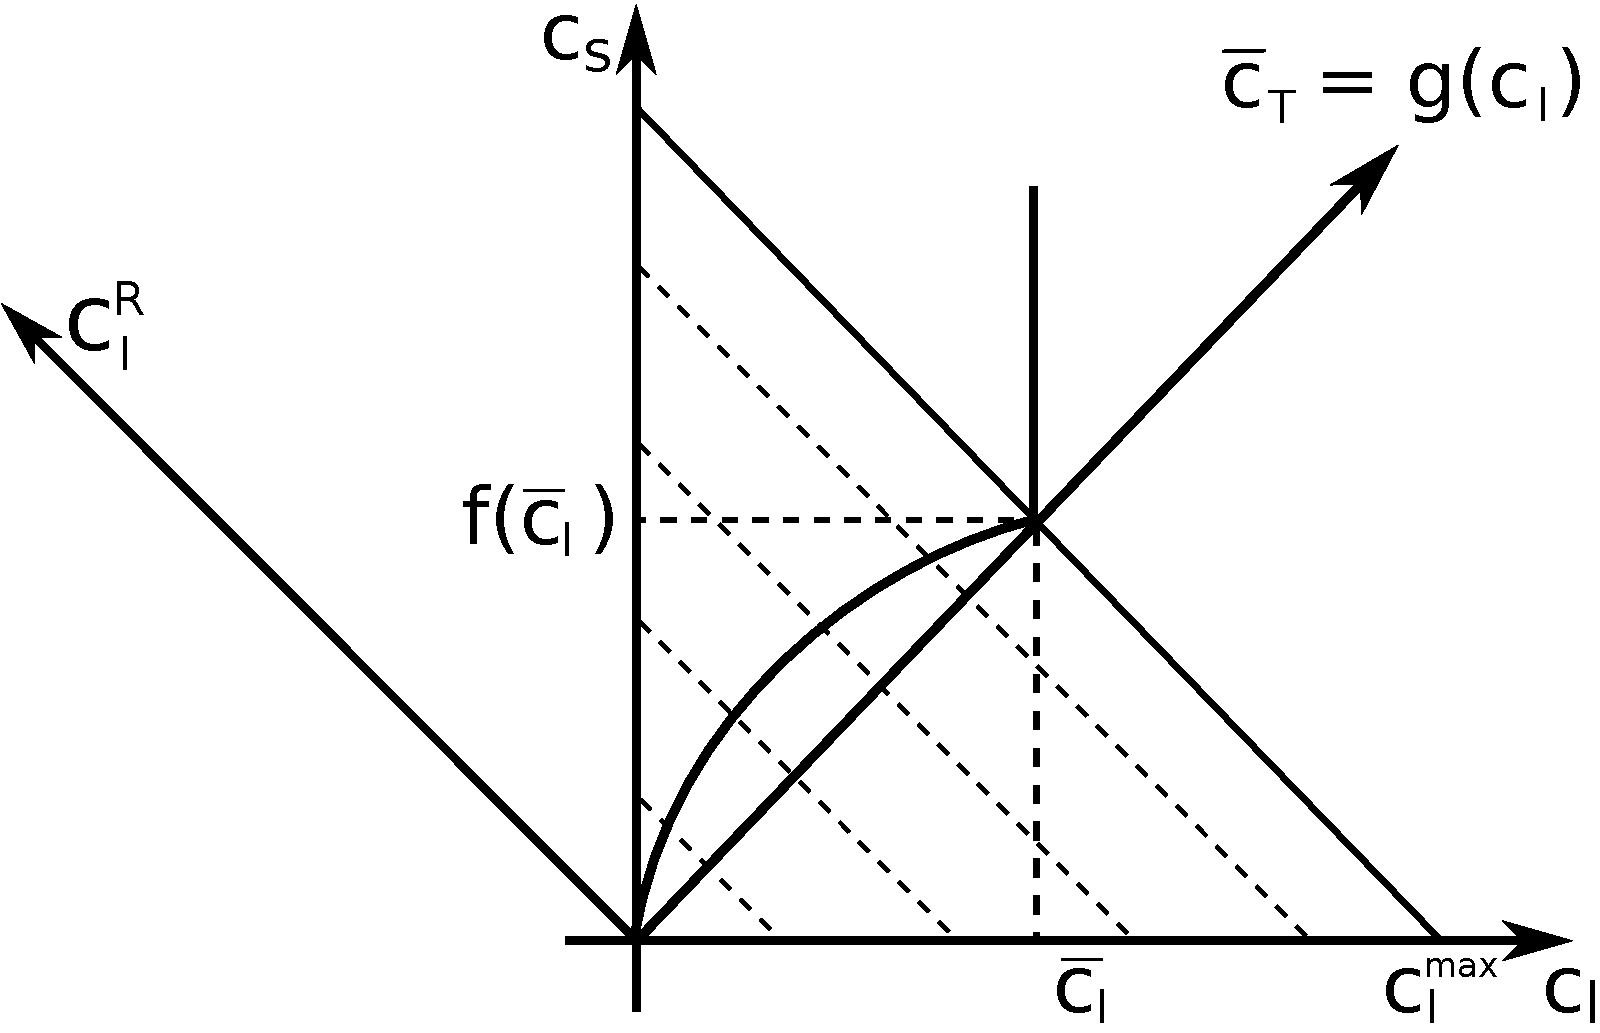
\includegraphics[width = 0.75\textwidth]{\fig/sorpce.pdf}
 \caption{Sorption in combination with limmited solubility.}
 \label{fig:sorpce}
\end{figure}


To approximate the equation \eqref{eq:nonlin_sorption} using interpolation, we need to prepare the set of values 
which represents $[c_l, f(c_l)]$, with $c_l$ equidistantly distributed in transformed (rotated and rescaled) 
coordination system at first. The construction process of the interpolation table follows.
\begin{enumerate}
 \item Maximal ``total mass'' $\bar{c}_T = \mu_l\cdot \bar{c}_l + \mu_s\cdot f(\bar{c}_l)$ is computed.
 \item Total mass step is derived $mass\_step = \bar{c}_T/n\_steps$. $n\_steps$ is given by
       \hyperA{Sorption::substeps}{$substeps$}.
 \item Appropriate $c_T^j = (mass\_step\cdot j)/\mu_l,~j\in \{0,\ldots, n\_steps\}$ are computed. 
 \item The equations $\mu_l \cdot c_T^j = \mu_l\cdot c_l^j + \mu_s\cdot f(c_l^j)~j\in \{0,\ldots, n\_steps\}$ are solved 
       for $c_l^j$ as unknowns. The solution is the set of ordered couples (points) 
       $[c_l^j,f(c_l^j)],~j\in\{0,\ldots,n\_steps\}$.
\end{enumerate}
After the computation of $\{[c_l^j,f(c_l^j)]\}$, we transform these coordinates to the system where the total mass is 
an independent variable. This is done by multiplication of precomputed points using the transformation matrix ${\bf A}$:
\begin{equation}
 \begin{array}{l}
  \vec{c}\,^R = {\bf A}\cdot\vec{c}\\
  \left[\begin{array}{c} c_l^{R,j}\\ c_s^{R,j} \end{array}\right] = 
  \left[\begin{array}{cc}
    \vartheta\cdot \rho_w & M_s(1 - \vartheta)\rho_R\\
    -M_s(1 - \vartheta)\rho_R & \vartheta\cdot \rho_w
  \end{array}\right]\cdot
  \left[\begin{array}{c} c_l^j\\ c_s^j \end{array}\right]\\
  j\in\{0,\ldots,n\_steps\}
 \end{array}
 \label{eq:transf_mat}
\end{equation}

The values $c_l^{R,j}$ are equidistantly distributed and there is no reason to save them, but the values 
$c_s^{R,j}$ are stored in onedimensional interpolation table.

Once we have the interpolation table, we can use it for projecting the transport results ${[c_l,c_s]}$ on the 
isotherm under consideration. Following steps must be taken.
\begin{enumerate}
 \item Achieved concentrations are transformed to the coordinate system through multiplication with the 
       matrix ${\bf A}$, see \eqref{eq:transf_mat}.
 \item Transformed values are interpolated.
 \item The result of interpolation is transformed back. The backward transformation consists of multiplication 
       with ${\bf A}^T$ which is followed by rescaling the result. Rescaling the result is necessary because  
       ${\bf A}$ is not orthonormal as it is shown bellow.
 \[
 \begin{array}{l}
 {\bf A}^T\cdot{\bf A} =
  \left((\vartheta - 1)^2\cdot M_s^2\cdot \rho_R^2 + \vartheta^2\cdot \rho_w^2\right)\cdot\left[\begin{array}{cc}
    1 & 0\\
    0 & 1
  \end{array}\right]
  \end{array}
 \]
\end{enumerate}


\subsection{Limited Solubility}\label{subsec:lim_solub}
When $\mu_l\cdot c_l + \mu_s\cdot f(c_l) > \mu_l\cdot \bar{c}_l + \mu_s\cdot f(\bar{c}_l)$ neither iterative 
solver nor interpolation table is used. The aqueous concentration is set to be $\bar{c}_l$ and sorbed 
concentration is computed $c_s = (\mu_l\cdot c_l + \mu_s\cdot f(c_l) - \mu_l\cdot \bar{c}_l)/\mu_s$.

\subsection{Sorption in Dual Porosity Model} 
\label{subsec:sorp_dual_por}
There are two parameters $\mu_l$ and $\mu_s$, scale of aqueous concentration and scale of sorbed concentration, respectively.  
There is a difference in computation of these in the dual porosity model because both work on different concentrations
and different zones.

Let $c_{ml}$ and $c_{ms}$ be concentration in liquid and in solid in the mobile zone, 
$c_{il}$ and $c_{is}$ be concentration in liquid and in solid in the immobile zone,
$\vartheta_m$ and $\vartheta_i$ be the mobile and the immobile porosity,
and $\varphi$ be the sorbing surface.

The sorbing surface in the mobile zone is given by
\begin{equation}
  \varphi = \frac{\vartheta_m}{\vartheta_m + \vartheta_i}, 
\end{equation}

while in the immobile zone it becomes
\[ 1 - \varphi = 1-\frac{\vartheta_m}{\vartheta_m + \vartheta_i} = \frac{\vartheta_i}{\vartheta_m + \vartheta_i}. \]

Remind the mass balance equation \eqref{eq:nonlin_sorption}.
In the dual porosity model, the scaling parameters $\mu_l$, $\mu_s$ are slightly different.
In particular, the mass balance in the mobile zone reads:
\begin{eqnarray}
 \begin{array}{l}
  c_T = \mu_l\cdot c_{ml} + \mu_s\cdot c_{ms},\\
  \mu_l = \varrho_l \cdot \vartheta_m, \\
  \mu_s = M_s \cdot\varrho_s\cdot(1-\vartheta_m - \vartheta_i)\varphi,
 \end{array}
 \label{eq:scale_params_m}
\end{eqnarray}
while in the immobile zone it has the form:
\begin{eqnarray}
 \begin{array}{l}
  c_T = \mu_l\cdot c_{il} + \mu_s\cdot c_{is},\\
  \mu_l = \varrho_l \cdot \vartheta_i, \\
  \mu_s = M_s \cdot\varrho_s\cdot(1-\vartheta_m - \vartheta_i)(1 - \varphi).
 \end{array}
 \label{eq:scale_params_i}
\end{eqnarray}
